% !TeX spellcheck = en_GB
%%%%%%%%%%%%%%%%%%%%%%%%%%%%%%%%%%%%%%%%%%%%%%%%%%%%%%%%%%%%%%%%%%%%%%%%%%%%%%%%
% Preamble                                                                     %
%%%%%%%%%%%%%%%%%%%%%%%%%%%%%%%%%%%%%%%%%%%%%%%%%%%%%%%%%%%%%%%%%%%%%%%%%%%%%%%%

\documentclass[12pt,a4paper,openbib]{report}

\usepackage{estilo_pfc}
\usepackage{longtable}
\usepackage{musixtex}
\usepackage{cite}
\usepackage{titlesec}
\usepackage{fancyvrb}
\usepackage[export]{adjustbox}
\usepackage{relsize}

\author{AUTOR/A DEL PROYECTO}
\date{FECHA DEL PROYECTO}

%%%%%%%%%%%%%%%%%%%%%%%%%%%%%%%%%%%%%%%%%%%%%%%%%%%%%%%%%%%%%%%%%%%%%%%%%%%%%%%%
% Body                                                                         %
%%%%%%%%%%%%%%%%%%%%%%%%%%%%%%%%%%%%%%%%%%%%%%%%%%%%%%%%%%%%%%%%%%%%%%%%%%%%%%%%

\begin{document}

 %%%%%%%%%%%%%%%%%%%%%%%%%%%%%%%%%%%%%%%%
 % Definición de comandos               %
 %%%%%%%%%%%%%%%%%%%%%%%%%%%%%%%%%%%%%%%%

 \newcommand{\paginaenblanco}{\mbox{}\thispagestyle{empty}\newpage}
 \newcommand{\exedout}{%
   \rule{0.8\textwidth}{0.5\textwidth}%
 }

 %%%%%%%%%%%%%%%%%%%%%%%%%%%%%%%%%%%%%%%%
 % Preliminares documento               %
 %%%%%%%%%%%%%%%%%%%%%%%%%%%%%%%%%%%%%%%%

 \begin{titlepage}
\begin{center}
\includegraphics[width=5cm]{imagenes/anagramaUDC.png}\\
{\textsc{Faculty of Computer Science}} \\ [2.5cm]
{\Large \textsc{Technical Report}} \\[0.5cm]
{\Large \textsl{\textbf{Haspie: A Musical Harmonization Tool}}} \\[0.15cm]
{\Large \textsl{\textbf{powered by Answer Set Programming}}} \\
\vfill
\begin{flushright}
\begin{tabular}{ll}
\textbf{Authors:}    & Martín Prieto, Rodrigo \\
 & Cabalar Fernández, José Pedro \\
& \\
\multicolumn{2}{r}{\small \emph{A Coruña, \today{}.}} \\
\end{tabular}
\end{flushright}
\end{center}
\end{titlepage}

 %%%%%%%%%%%%%%%%%%%%%%%%%%%%%%%%%%%%%%%%%%%%%%%%%%%%%%%%%%%%%%%%%%%%%%%%%%%%%%%%

\begin{abstract}
\thispagestyle{empty}
Este proyecto consiste en el desarrollo de una herramienta inteligente de ayuda a la armonización capaz de comprender la armonía presente en una partitura y completar tramos de la misma, llegando incluso a poder crear nuevas voces de la nada que sean correctas desde un punto de vista armónico. Esto puede servir como una herramienta individual para ayudar al estudiante de armonía a comprender mejor la materia o al compositor novel a explorar nuevas soluciones a la hora de incluir secciones en su pieza, o también puede servir como utilidad intermedia para ser combinada con otras herramientas de creación o edición musical. Pese a que el fin del proyecto es crear la herramienta en sí, sirve también como demostración empírica de la aplicabilidad de las técnicas de \textit{Answer Set Programming} al campo de la música. 
\end{abstract}

%%%%%%%%%%%%%%%%%%%%%%%%%%%%%%%%%%%%%%%%%%%%%%%%%%%%%%%%%%%%%%%%%%%%%%%%%%%%%%%%

 \thispagestyle{empty}
\begin{description}
 \item [Palabras clave:] \mbox{} \\
   \begin{list}{$\surd$}{}
     \item Programación Declarativa
     \item Programación Lógica
     \item Procesamiento de Lenguajes
     \item Representación del Conocimiento
     \item Answer Set Programming
     \item Música
     \item Música por computador
     \item Armonía
     \item clingo
     \item MusicXML
   \end{list}
\end{description}


 \pagenumbering{roman}
 \setcounter{page}{1}

 \tableofcontents
 \listoffigures
 \clearpage
 \mbox{}
 \clearpage

 \pagenumbering{arabic}
 \setcounter{page}{1}

 %%%%%%%%%%%%%%%%%%%%%%%%%%%%%%%%%%%%%%%%
 % Capítulos                            %
 %%%%%%%%%%%%%%%%%%%%%%%%%%%%%%%%%%%%%%%%

 \chapter{Introduction}
\label{chap:introduction}

%%%%%%%%%%%%%%%%%%%%%%%%%%%%%%%%%%%%%%%%%%%%%%%%%%%%%%%%%%%%%%%%%%%%%%%%%%%%%%%%
% Objetivo: Exponer de qué va este proyecto, sus líneas maestras, objetivos,   %
%           etc.                                                               %
%%%%%%%%%%%%%%%%%%%%%%%%%%%%%%%%%%%%%%%%%%%%%%%%%%%%%%%%%%%%%%%%%%%%%%%%%%%%%%%%

\lettrine{M}usic Theory learning has been stuck in the same old-fashioned methods and systems for years. These methods are based on exercises and repetition, meant to train the ear and become fluent in composition or in solving the proposed exercises. Harmony learning is one of the most important steps in music, since being able to analyse scores in this way is vital for its comprehension, later interpretation and further development. Haspie aims to help Harmony students achieve a better understanding of the matter and lets them experiment earlier with composition from an harmonic point of view.

Constraint Logic fits well with the problem since the harmony rule set used in the most basic levels taight in music schools hasn't changed since the origins of the subject, it's a definite set of rules, not very big and quite strict. Simply translating this rule set to ASP constraints and being able to extract the fatcs and knowledge from any score, the tool is able to detect any mistake and propose solutions, as well as filling in any blank sections of the score to create, in the end the harmony of the piece.

The great advantage that Answer Set Programming provides is that there is no need to create nor optimise a solution searching algorithm, since it only needs these harmony rules. Answer Set Programming not only offers this simplicity and power, but also flexibility since a change in the rules or in the optimization configuration can lead to very different results and adapt better to the composition style of the user.

 

 \chapter{Background}
\label{chap:background}
\vspace{0.5cm}

%%%%%%%%%%%%%%%%%%%%%%%%%%%%%%%%%%%%%%%%%%%%%%%%%%%%%%%%%%%%%%%%%%%%%%%%%%%%%%%%
% Objetivo: Contar cómo estaba la situación antes de empezar,                  %
%           todo lo que se hizo para familiarizarse con las tecnologías,       %
%           casarlas, etc.                                                     %
%%%%%%%%%%%%%%%%%%%%%%%%%%%%%%%%%%%%%%%%%%%%%%%%%%%%%%%%%%%%%%%%%%%%%%%%%%%%%%%%

\section{State of the Art}
\label{sec:state-of-the-art}

\lettrine{L}a mayor parte del trabajo en la creación y composición musical en ordenadores se ha extraído de la relación entre la teoría musical y las matemáticas. No es difícil concluir que la música y sus reglas son fácilmente modelables de forma matemática. 

Dentro de la música en computación existen varias ramas diferenciadas, aunque en el contexto de un mismo trabajo pueden verse mezcladas más de una. Hablamos de composición asistida y de de sistemas inteligentes orientados a composición y, aunque se tratarán con más detalle en los siguientes puntos, todos ellos, así como el software desarrollado en dichos campos, están destinados a la creación y composición musical. Se detallan, además, algunos de los formatos más comunes de representación musical.

Si bien el sistema planteado en el proyecto no es un compositor, se enmarca dentro de este mismo contexto, y por tanto es necesario desglosarlo para entender en qué punto se encuentra la tecnología desarrollada en el momento de la publicación de este documento.

\subsection{Answer Set Programming}
\label{subsec:asp}
El módulo principal del proyecto se ha desarrollado usando técnicas conocidas como \textit{Answer Set Programming}\cite{Brewka:2011:ASP:2043174.2043195} (ASP de ahora en adelante) basadas en modelos estables de Gelfond \& Lifschitz\cite{Gelfond88thestable} y lógica no-monótona. ASP es un lenguaje de programación declarativa orientado a problemas de búsqueda difíciles, principalmente NP-complejos. ASP ha demostrado ser particularmente útil en aplicaciones donde es necesaria la representación del conocimiento y el razonamiento a partir de dicho conocimiento. En ASP, los problemas de búsqueda se reducen al cómputo de modelos estables, usándose programas conocidos como\textit{solvers} para realizar la búsqueda de las soluciones. El lenguaje de entrada de ASP es una variante enriquecida del lenguaje prolog. Para traducir el lenguaje de entrada a reglas de programación declarativa convencional y poder construir los modelos estables subyacentes del problema, ASP cuenta con \textit{grounders} que se encargan de esta transformación.

La implementación de un programa que busque soluciones a un problema concreto pasa por la definición de las reglas de ese problema de modo general, mientras que la definición del problema concreto a solucionar se especifica mediante hechos lógicos que, en combinación con las reglas generales del problema generan todas las posibles soluciones del mismo. Finalmente, estas soluciones se podan mediante restricciones lógicas y/o restricciones de cardinalidad. Este proceso constituye la metodología general del desarrollo en ASP, conocida como \textit{generate and test}

Las herramientas desarrolladas por el grupo Potassco\footnote{http://potassco.sourceforge.net/} incluyen, entre otras, un \textit{grounder} (Gringo) y un \textit{solver} (Clasp), junto con una herramienta única que combina ambos llamada Clingo.

\begin{itemize}
 \item \textbf{Gringo} es el \textit{grounder} de la suite. Se encarga de transformar reglas generales a reglas concretas y transforma el problema planteado a un lenguaje entendible por el \textit{solver}.
 \item \textbf{Clasp} es el \textit{solver} de la suite. Se encarga de decidir el conjunto final de soluciones válidas dado el problema procesado e interpretado por el \textit{grounder}.
 \item \textbf{Clingo} es una herramienta combinada formada por clasp y gringo. Realiza el procesado completo de un problema planteado en ASP y permite indicar algunas preferencias adicionales.
\end{itemize}

\subsection{Formatos}
\label{subsec:formats}
Debido al contexto en el que se enmarca este proyecto no se cree necesario considerar formatos de salida finales, como OGG, WAV o MP3 ya que como su nombre indica, son formatos utilizados solo para reproducción que no permiten extraer ni editar información musical de forma precisa. Así mismo tampoco se contemplan formatos de representación de partituras en forma de imágenes como SVG, PNG o PDF por motivos similares.

\subsubsection{MusicXML}
MusicXML, MXML o \textit{Music Extensible Markup Language} es una extensión del formato XML usado en la representación de música occidental. No solo contiene información musical sino que también incluye información de su representación en papel, tal como márgenes, tamaños de fuente, posición de las notas en coordenadas, etc. Hace uso del sistema de etiquetas anidadas de XML para agrupar los diferentes bloques de información de una pieza, como las voces, los compases o la información individual de cada nota (Ver Figura \ref{fig:nota_musicxml}). Es un formato muy rico aunque difícil de escribir correctamente a mano. Es por esto que normalmente se usa solo como formato de intercambio entre software que lo acepta como entrada o salida.

\begin{figure}[h!]
	\centering
	\begin{Verbatim}[frame=single]
<note default-x="74.65" default-y="-25.00">
	<pitch>
		<step>A</step>
		<octave>4</octave>
	</pitch>
	<duration>1</duration>
	<voice>1</voice>
	<type>quarter</type>
	<stem>up</stem>
</note>
	\end{Verbatim}
	\caption{Ejemplo de nota representada en MusicXML}
	\label{fig:nota_musicxml}
\end{figure}


\subsubsection{LilyPond}
LilyPond\footnote{http://www.lilypond.org/} es un conjunto formado por el software y el formato de fichero homónimos. LilyPond como formato usa su propio lenguaje de marcado. Las etiquetas de LilyPond se parecen más a las usadas en \LaTeX. De forma similar a MusicXML, incluye información de representación final, aunque en mucha menor cantidad (Sólo tamaño de papel, márgenes o sangrados). La información musical de la canción está anidada por secciones de forma similar a MusicXML, aunque ésta se organiza de forma mucho más intuitiva para el lector humano del fichero (Ver Figura \ref{fig:partitura_lilypond}). Es un formato ligero pensado para poder ser editado a mano, aunque la mayoría del software musical actual lo soporta como entrada y salida. 

El software del mismo nombre es un programa de grabado musical (tipografía musical o edición de partituras), pensado para producir partituras de alta calidad. Lleva la estética de la música tipografiada de la forma tradicional a las partituras impresas mediante ordenador. LilyPond es software libre y forma parte del Proyecto GNU. 

\begin{figure}[h!]
	\centering
\begin{Verbatim}[frame=single]
\version "2.14.1"
{
	<c' d'' b''>8. ~ <c' d'' b''>8
}
\end{Verbatim}
	\caption{Ejemplo de una pequeña pieza musical en lilypond}
	\label{fig:partitura_lilypond}
\end{figure}



\subsubsection{MIDI}
MIDI son las siglas de \textit{Musical Instrument Digital Interface}. Es un standard técnico compuesto de un protocolo, una interfaz digital y conectores que permiten a una gran variedad de instrumentos electrónicos, ordenadores y otros dispositivos conectarse y comunicarse entre sí, principalmente con fines musicales, pero no siempre.

MIDI transmite mensajes de eventos que especifican notación, tono y velocidad, aunque también incluye información de modificaciones sobre estos sonidos como volumen, \textit{vibrato} y marcas de tiempo para sincronizar entre dispositivos. 

Estos mensajes pueden ser codificados en ficheros para reproducción, edición o simplemente como formato de representación musical pudiendo ser editado posteriormente. Dado que no contiene información final de audio, MIDI supone una gran ventaja en cuanto a espacio en disco, aunque el sonido final depende del equipo que reproduzca el fichero.


\subsection{Software}
\label{subsec:software}
\subsubsection{Herramientas}
\begin{itemize}
	\item \textbf{Flex y Bison} son utilidades Unix que permiten escribir \textit{parsers} veloces para casi cualquier formato de archivo. Implementan procesado \textit{Look-Ahead-Left-Right} de gramáticas libres de contexto no ambiguas.
	\item \textbf{Music21} es un conjunto de herramientas que sirve de ayuda a estudiantes y músicos a responder preguntas sobre música rápida y eficazmente. No sólo posee una base de datos bastante completa para realizar análisis musicológicos sino que contiene herramientas para la composición programática de música.
\end{itemize}

\subsubsection{Composición Asistida}
Dentro de la composición asistida encontramos principalmente software de composición general en forma de editores de partituras que incorporan herramientas para ayudar al compositor en el proceso. Estas herramientas pueden ser corrección de la métrica de los compases, transposición de secciones de la canción, cambios de tonalidad, construcción de acordes dada una nota generadora, etc.

\begin{itemize}
 \item \textbf{Musescore 2} es un editor \textit{WYSIWYG} capaz de exportar a varios formatos de representación musical digital, tales como MIDI, LilyPond o MusicXML.
\item \textbf{Sibelius} permite trabajar con gran variedad de modos de entrada de notas para sus partituras, desde los formatos convencionales hasta a través de instrumentos con salida MIDI o mediante el escaneado de partituras en papel haciendo uso de OCR.
\item \textbf{Finale} destaca por la cantidad de ajustes que permite realizar sobre el pentagrama a un nivel de detalle muy fino, aunque presenta una curva de aprendizaje muy elevada. Sus principales características  tienen que ver con la visualización del pentagrama, ya que posee \textit{plug-ins} que se encargan de que el espacio entre las notas sea el correcto o que no haya colisiones entre notas de diferentes voces entre otros. 
\end{itemize}


\subsubsection{Sistemas Inteligentes}
Aunque la música puede modelarse de forma matemática, con reglas estrictas que derivan en algoritmos de composición, también requiere creatividad. Un algoritmo determinista no puede ser creativo, ya que para la misma entrada, siempre producirá la misma salida. Si bien existe la composición algorítmica como aproximación a la música compuesta por ordenadores, no es relevante para este trabajo.

Dentro de la inteligencia artificial, se han realizado aproximaciones a la composición musical desde gran parte de las ramas principales del campo

\begin{itemize}
	\item \textbf{EMI y Emily Howell} Desarrollado por David Cope\cite{experiments-musical-intelligence}, EMI o Experiments in Music Composition, es un sistema capaz de identificar el estilo presente en una partitura incompleta y completar la cantidad de notas restantes que el compositor requiera. El trabajo de Cope estudia la posibilidad de emplear gramáticas y diccionarios en la composición musical. EMI derivó en el software Emily Howell.
	Emily Howell utiliza EMI para crear y actualizar su base de datos, pero cuenta con una interfaz a través de la cual se puede modificar, a través de \textit{feedback}, la composición. Cope enriqueció y pulió Emily Howell con su propio estilo musical para crear varios discos que después fueron publicados.
	\item \textbf{ANTON}\cite{anton-composing} es un sistema de composición rítmica, melódica y armónica basado en Answer Set Programming. ANTON compone breves piezas musicales desde cero o partiendo de partituras incompletas utilizando un estilo basado en el del compositor renacentista Giovanni Pierluigi da Palestrina. Recibe como entrada ficheros con las notas codificadas como hechos lógicos para después rellenar las secciones incompletas o añadir nuevas notas hasta que la pieza está completa. ANTON crea y completa dichas piezas teniendo en cuenta el número de tiempos rítmicos de las mismas y seleccionando la nota correspondiente de acuerdo a la nota  o estado anterior.
	\item \textbf{Vox Populi}\cite{vox-populi} utiliza algoritmos evolutivos para componer música en tiempo real. En este sistema, se parte de una población de acordes codificados mediante el protocolo MIDI para después mutarlos y seleccionar los mejores acordes a criterios puramente físicos relevantes para la música. Su interfaz gráfica permite al usuario controlar la función de \textit{fitness} del proceso evolutivo así como los atributos del sonido producido.
	\item \textbf{CHORAL} es un sistema experto que funciona como armonizador en el estilo clásico de Johann Sebastian Bach. Las reglas que utiliza el sistema representan conocimiento musical desde varios puntos de vista de la coral. El programa armoniza melodías corales mediante un sistema de generación y prueba con \textit{backtracking}. La base de conocimiento de CHORAL permite realizar modulaciones propias del estilo, crear patrones rítmicos e impone restricciones complejas para mantener el interés melódico en las voces intermedias.
	\item \textbf{CHASP} es una herramienta creada por el grupo Potassco para calcular progresiones de acordes mediante Answer Set Programming partiendo de cero, pudiendo especificar clave y duración. A diferencia del presente proyecto no toma un fichero de entrada para armonizar piezas, pero sí que es capaz de dotar a la salida del programa de diferentes estilos rítmicos.
\end{itemize} 





 \chapter{Method}
\label{chap:desarrollo}
\vspace{0.5cm}

%%%%%%%%%%%%%%%%%%%%%%%%%%%%%%%%%%%%%%%%%%%%%%%%%%%%%%%%%%%%%%%%%%%%%%%%%%%%%%%%
% Objetivo: Exponer las partes relevantes de la implementación                 %
%%%%%%%%%%%%%%%%%%%%%%%%%%%%%%%%%%%%%%%%%%%%%%%%%%%%%%%%%%%%%%%%%%%%%%%%%%%%%%%%

\section{Approach}
\label{sec:metodology}

The architecture of \texttt{haspie} (See Figure \ref{fig:arquitectura_final}) is a simple pipeline wirtten in Python with a single execution path. This pipeline calls each submodule passing the correct parameters and then retrieves and parses the output generated by each step of the tool.

\begin{figure}[h]
	\centering
	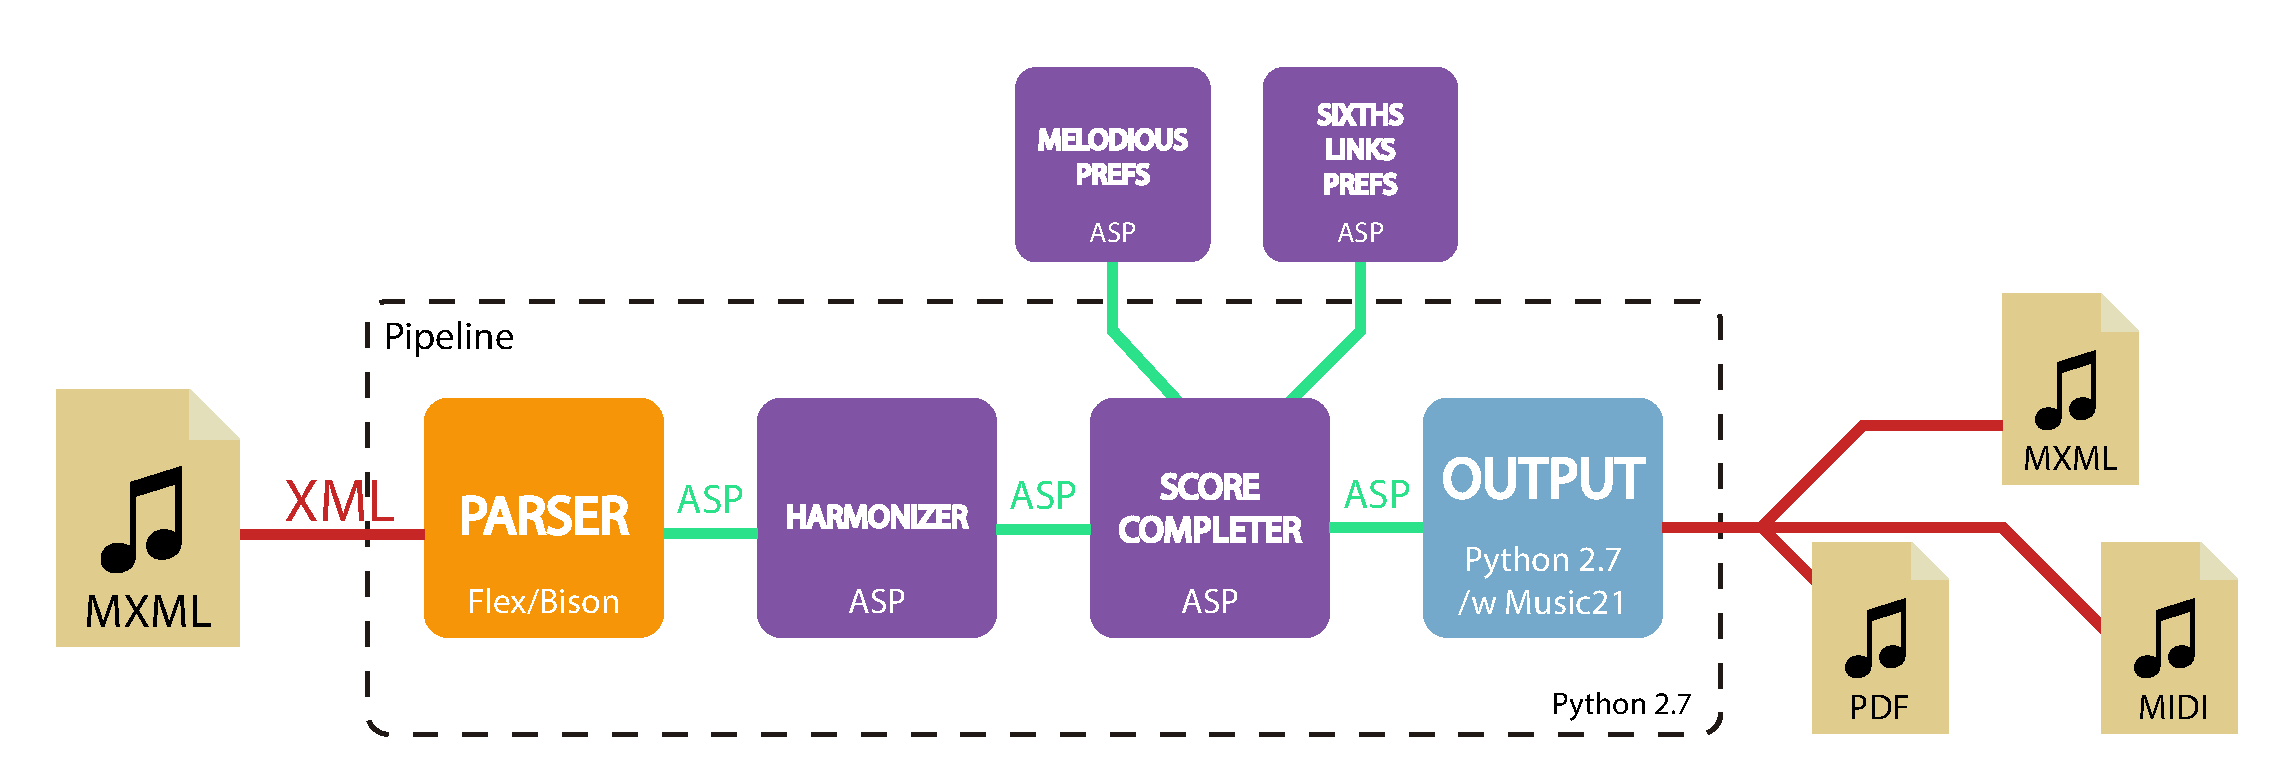
\includegraphics[width=0.8\linewidth]{imagenes/arquitectura_final.pdf}
	\caption{Haspie's Architecture}
	\label{fig:arquitectura_final}
\end{figure}

\subsection{Input}
The tool takes a single MusicXML file as input that is passed to the first stage of the pipeline: a parser written in C along with the Flex and Bison libraries. This module transforms the MusicXML tag information to Answer Set Programming logic facts. This parser does not only parse the musical figures but also performs many other tasks such as:

\begin{itemize}
 	\item Subdividing the figures to standardize the rhythmic patterns.
 	\item Creating additional logic facts to retrieve the original rhythm structures after the score processing.
 	\item Identifying the different measure types.
 	\item Interpreting the instrument names to determine their most common pitch ranges.
 	\item Infer the tonality of the score by parsing it's key.
 	\item Parsing some of the score metadata, such as the piece name or the composer.
\end{itemize}

After the parsing step, all of this extracted data is saved in the form of configuration and answer set programming files. (See Figure \ref{fig:simple-piece-facts})

\begin{figure}[h]
	\centering
	\includegraphics[width=0.4\linewidth]{imagenes/example_notes.png}
	\includegraphics[width=0.3\linewidth]{imagenes/logic_facts_score.png}
	\caption{Small piece parsed to ASP facts}
	\label{fig:simple-piece-facts}
\end{figure}

\subsection{ASP Core}
The previously created ASP fact file is the direct input of the harmonization finder step, which is the first half of haspie's ASP Core.
These module uses these facts to expand the general harmony rules, thus inferring support hidden predicates and finally assigning a chord to each specified section of the piece.

\begin{Verbatim}[frame=single]
1 { chord(HT,C) : pos_chord(C) } 1 :- htime(HT).
\end{Verbatim}

The possible chords are defined in separate files \texttt{major\_chords} and \texttt{minor\_chords}, the tool determines which to use by inferring the mode from the extracted key. These chords are defined by the tonal relation between their notes and not by their notes particular name. By doing it this way, the tool generalizes the chord concept, reducing it to a tonal grade detection and then fitting the best possible chord for that grade by taking all the notes in the analyzed beat interval. To do so, the parsed notes' pitches are abstracted to tonal grades of the corresponding scale (using the inferred key). This is achieved by performing simple operations to the note's semitone value.

\begin{Verbatim}[frame=single]
octave(V,((N - base) / 12),T) :- note(V,N,T), N >= 0.
sem_tones(V,((N - base) \ 12),T) :- note(V,N,T), N >= 0.
grade(V,1,T) :- sem_tones(V,3,T).
grade(V,2,T) :- sem_tones(V,5,T).
grade(V,3,T) :- sem_tones(V,7,T).
grade(V,4,T) :- sem_tones(V,8,T).
grade(V,5,T) :- sem_tones(V,10,T).
grade(V,6,T) :- sem_tones(V,0,T).
grade(V,7,T) :- sem_tones(V,2,T).
\end{Verbatim}

Knowing the tonal grades of each note of the rhythmic interval, the tool then marks the notes in strong beats as mistakes and, by the use of optimization rules, searches the answer that minimizes the amount of mistakes


\begin{figure}[h]
	\centering
	\includegraphics[width=0.4\linewidth,valign=c]{imagenes/harmonized_example.png}
	\includegraphics[width=0.2\linewidth,valign=c]{imagenes/chord_facts.png}
	\caption{Chords annotated over a small piece and their corresponding output logic facts}
	\label{fig:simple-piece-chords}
\end{figure}

Back to the pipeline, the best possible found harmonies are parsed to an object Python representation that makes possible their future representation and music score recomposition. The tool displays a summary of these best answers and lets the user choose one for the completion step, by default the tool uses the solution with least mistakes in it's harmonization. A temporal chord facts file is then created, that is used, along with the original logic facts to complete the blank parts or the new voices of the score. (See Figure \ref{fig:simple-piece-chords})

The second half of the tool is called if there are blank sections in the score or the creation of new parts were specified to the pipeline. This second half works in a similar fashion as the first half, by assigning new notes to the completable sections of the score among the pitch range of the specified instrument or voice type of the part.

\begin{Verbatim}[frame=single]
1 { freebeatfigure(V,N,1,FB) : N=VL..VH } 1 :- freebeat(V,FB),
		voice_limit_low(V,VL), voice_limit_high(V,VH).
\end{Verbatim}

These new notes are again generalized to their tonal grade and octave (as it's done in the very first steps of the previous half) to then being checked against the selected harmonization. This is done by marking the incorrect ones in strong beats as mistakes, as well as checking for other melodic rules such as note distance or trying to avoid certain undesirable sounds produced among the different voices that play at the same time. By minimizing these mistakes, again, the optimal solutions are found.
	\begin{Verbatim}[frame=single]
octave_jump(V,B1,B2) :- ex_note(V,N1,B1), ex_note(V,N2,B2),
          	 (B1+1) == B2, N2 > (N1+12), beat(B1+1).
octave_jump(V,B1,B2) :- ex_note(V,N1,B1), ex_note(V,N2,B2),
           	(B1+1) == B2, N2 < (N1-12), beat(B1+1).
:- octave_jump(_,_,_).
	\end{Verbatim}

Finally, thanks to the extra rhythmical predicates extracted by the parser, the original piece is reconstructed.

\begin{figure}[h]
	\centering
	\includegraphics[width=0.35\linewidth,valign=c]{imagenes/incomplete_score.png}
	\includegraphics[width=0.3\linewidth,valign=c]{imagenes/incomplete_facts.png}
	\includegraphics[width=0.35\linewidth]{imagenes/completed_score.png}
	\caption{Completed harmonized score with an incomplete beat}
	\label{fig:simple-piece-complete}
\end{figure}

Repeating the previous process, the user chooses a complete score solution and then the pipeline stores the new information in object structures for their final file output in the specified format. (See Figure \ref{fig:simple-piece-complete})

\subsection{Preferences Modules}
Haspie has two optional preferences modules that add some further rules to improve the second half of the ASP core results.

The first one is a melodic preference module. As haspie does not have a well-defined composition rule set, this module aims to smoothen the completed blank sections of the score. It has rules for:
\begin{itemize}
	\item Defining the melody tendency
	\item Shortening the melodic jumps between notes
\end{itemize}

For tendency, the rules infer if a section has a rising or falling tendency and tries to imitate that tendency in the completable sections. For the melodic jump smoothening, new predicates infer these jump sizes and optimization rules search for the solutions that minify these jumps.

\begin{Verbatim}[frame=single]
melodic_jump(V,J,B1,B2) :- out_note(V,N1,B1), out_note(V,N2,B2),
             	(B1+1) == B2, beat(B1+1), J = #abs(N1-N2). 
\end{Verbatim}

The second module detects certain popular choral chord progressions (fourth and sixth inversions) and try to complete them by selecting the correct notes for them in the completable blank sections. These module performs a second per-beat harmonization, making it very slow computationally.

Haspie contains a standard configuration files that weight both these preference modules and the both halves of the core optimization values. By changing these values, the harmonization and composition results may be altered, making it easier for the user to change the way the tool works without having to implement or modify new ASP rules or preference modules.

\subsection{Output}
The last module called by the pipeline uses the score's internal representation Python objects to export the result in the format specified by the user. This module works using the music21 library \footnote{http://web.mit.edu/music21/} developed by the MIT. The internal structure is translated to this library own object representation to then being exported easily to any of the supported formats.

\begin{figure}[h]
	\centering
	\includegraphics[width=0.4\linewidth]{imagenes/example_final_score.png}
	\caption{Sample harmonized score tih passing notes marked in blue}
	\label{fig:simple-piece-final}
\end{figure}



 \chapter{Evaluación}
\label{chap:evaluation}
\vspace{0.5cm}

%%%%%%%%%%%%%%%%%%%%%%%%%%%%%%%%%%%%%%%%%%%%%%%%%%%%%%%%%%%%%%%%%%%%%%%%%%%%%%%%
% Objetivo: Exponer los resultados objetivos del sistema                       %
%%%%%%%%%%%%%%%%%%%%%%%%%%%%%%%%%%%%%%%%%%%%%%%%%%%%%%%%%%%%%%%%%%%%%%%%%%%%%%%%

 \lettrine{E}{n} este capítulo exponen los resultados de la evaluación del sistema. Se han seleccionado tres piezas musicales conocidas para realizar las diferentes pruebas. A continuación se describen las tres piezas y las pruebas realizadas. Para realizar una prueba de carga que establezca los límites del sistema se ha añadido una última partitura suficientemente sencilla sobre la que trabajar para poder realizar estas pruebas cómodamente sin preocuparse por la calidad de los resultados.
 
 \begin{itemize}
 	\item \textbf{Menuet:} Famosa pieza de Johann S. Bach, destaca por su simpleza y es interesante para ver como funciona el programa ante compases ternarios. Se sugiere añadir una voz nueva de tesitura más aguda a la presente en la pieza.
 	\item \textbf{Greensleves:} Supuestamente compuesta por Enrique VIII, esta archiconocida partitura presenta una polifonía coral a cuatro voces, ideal para comprobar las capacidades de armonización del sistema. Se sugiere eliminar secciones grandes de la voz solista y ver cómo la completa.
 	\item \textbf{Joy to the World:} Conocido villancico, sería interesante escuchar una reinterpretación de la voz más grave para la pieza, ya sea completando secciones o bien añadiendo una voz de bajo.
    \item \textbf{Twinkle Twinkle Little Star:} Esta sencilla pieza tradicional infantil es adecuada para realizar, además de pruebas similares a otras piezas, pruebas de carga para comprobar como crecen los tiempos de búsqueda y hallar los límites de la herramienta.
 \end{itemize}
 
 Para la evaluación se han realizado armonizaciones de todas las piezas y se han medido los tiempos y la calidad de las mismas, además se han realizado pruebas de completado de un compás en cada pieza junto con la inclusión de una nueva voz, también se han medido calidad y tiempo. Por último, con la última partitura se han realizado pruebas para comprobar hasta donde funciona bien en cuestión temporal, para ello se ha ido vaciando porcentualmente una de las voces para ser completada y después se han ido añadiendo diferentes voces.
 
 Nótese que debido al carácter no-determinista de \textit{Answer Set Programming} y a los tiempos de entrada y salida estos tiempos sirven para dar una idea aproximada de los tiempos de funcionamiento de la herramienta. Para suavizar los valores dispares se ha ejecutado cada medida 100 veces, se ha restado el tiempo de usuario y se ha calculado el tiempo promedio. 
 
 \begin{figure}
 	\centering
 	\includegraphics[width=0.8\linewidth]{imagenes/evaluation/greensleeves_orig.png}
 	\caption{Comienzo de Greensleeves sin armonizar}
 	\label{fig:greensleeves_orig}
 \end{figure}
 
  \begin{figure}
  	\centering
  	\includegraphics[width=0.8\linewidth]{imagenes/evaluation/greensleeves_harm.png}
  	\caption{Comienzo de Greensleeves armonizado}
  	\label{fig:greensleeves_harm}
  \end{figure}
  
   \begin{figure}
   	\centering
   	\includegraphics[width=0.8\linewidth]{imagenes/evaluation/menuet_orig.png}
   	\caption{Comienzo de Menuet sin armonizar}
   	\label{fig:menuet_orig}
   \end{figure}
   
    \begin{figure}
    	\centering
    	\includegraphics[width=0.8\linewidth]{imagenes/evaluation/menuet_harm.png}
    	\caption{Comienzo de Menuet armonizado}
    	\label{fig:menuet_harm}
    \end{figure}
     \begin{figure}
     	\centering
     	\includegraphics[width=0.8\linewidth]{imagenes/evaluation/joy_orig.png}
     	\caption{Comienzo de Joy to the World sin armonizar}
     	\label{fig:joy_orig}
     \end{figure}
  
        \begin{figure}
        	\centering
        	\includegraphics[width=0.8\linewidth]{imagenes/evaluation/joy_harm_err.png}
        	\caption{La salida de Joy to the World produce un error de clave en la voz de la Soprano}
        	\label{fig:joy_harm_err}
        \end{figure}
     
      \begin{figure}
      	\centering
      	\includegraphics[width=0.8\linewidth]{imagenes/evaluation/joy_harm.png}
      	\caption{Comienzo de Joy to the World armonizado}
      	\label{fig:joy_harm}
      \end{figure}
  
  \begin{center}
  	\begin{tabular}{ | l | c | c | c | }
  		\hline
  		Pieza & T. Armonización & T. Compás & T. Nueva voz \\ \hline \hline
  		Greensleeves & 0.5922s & 0 & 0 \\ \hline
  		Menuet & 0.912s & 0 & 0 \\ \hline
  		Joy to the World & 4.378s & 0 & 0 \\ \hline
  		Twinkle Twinkle & 0s & 0 & 0 \\ \hline
  	\end{tabular}
  \end{center}
  
  \section{Problemas conocidos}
  \label{sec:known_issues}
  Las diferentes pruebas han revelado ciertos problemas que se producen si no siempre, sí lo hacen con una frecuencia relativamente alta y que por diseño de la herramienta no han sido atacados. En la sección de \ref{sec:future_work} Trabajo Futuro en el catulo \ref{chap:conclusiones} Conclusion se detalla cuales de ellos se pretenden arreglar a corto o medio plazo.
  
  \begin{itemize}
  		\item \textbf{Tresillos:} Los tresillos, dosillos y otras figuras irregulares no funcionan correctamente en la herramienta y han de ser editados en la partitura antes de procesarla. Esto se debe a que no es posible realizar una subdivisión directa a la nota base de la partitura de este tipo de figuras.
  		\item \textbf{Clave:} Algunas voces aparecen en la salida con la clave mal identificada, produciendo un resultado poco legible. Esto es fácilmente solucionable cambiando la clave de la voz correspondiente en el archivo de salida, ya que pese a todo, esto es un fallo meramente visual y no afecta a los valores de las notas de la voz.
  		\item \textbf{Nombres de Tesituras:} Si bien los nombres de las voces corales no varían sustancialmente, los nombres de los instrumentos sí lo hacen, por esto el \textit{locale} de la herramienta usada para la edición de partituras puede producir incompatibilidades a la hora de restringir el rango de voces, por ejemplo, una partitura para escrita para Violonchelo en un sistema en castellano marcará esa voz como \texttt{voice\_type(x, violonchelo)} mientras que un sistema en inglés producirá  \texttt{voice\_type(x, violoncello)}. Para solucionarlo se ruega editar el fichero \texttt{voice\_types.lp} en la carpeta \texttt{asp/include} para que los límites de cada instrumento se correspondan con el locale del sistema.
  		\item \textbf{Falsos positivos:} Debido a que en algunas figuras como los conjuntos de corcheas o semicorcheas consecutivas no se puede identificar los subtiempos débiles y fuertes que no dependen del compás si no de la propia figura junto con algunas dificultades a la hora de identificar los tiempos débiles y fuertes de un compás con las notas subdivididas y después transformarlo a otro tipo de compás, es probable que algunas notas marcadas como error en la partitura no lo sean realmente.
  \end{itemize}
  



 %%%%%%%%%%%%%%%%%%%%%%%%%%%%%%%%%%%%%%%%
 % Apéndices, glosarios y bibliografía  %
 %%%%%%%%%%%%%%%%%%%%%%%%%%%%%%%%%%%%%%%%
 \appendix
 \newpage

\chapter{Installation}
\label{chap:installation}
In it's current state, it's advised to install the tool in a Linux environment. This is mostly because of the use of Flex and Bison libraries, that are easily compiled and used in that kind of environments.

The requirements are Python 2.7 and the latest versions of Flex and Bison (as well as a C compiler). Other than that, gringo 3.0.5 and clingo 3.0.5 are needed, those can be downloaded at the Potassco Group's Sourceforge page \cite{potasscoweb} as well as the music21 module in it's latest version. All these tools and libraries should be accessible on the System's \texttt{PATH}

It is advised to install any tools required to compile or visualize the desired output formats before installing music21 so it can be properly attached to them without any further configuration.

Of course a score edition tool is also advised, it is completely optional but it's convenient. Musescore2 was used for the tests and demos as it's Open Source and free, but any other similar editor that can handle MusicXML files will work.

The tool can finally be executed by calling it's main entry point on a command line, and any of the parameters as well as it's usage explanation can be checked with the \texttt{-h} or \texttt{--help} options.

 \nocite*
 \bibliography{bibliography}
 \bibliographystyle{IEEEtran}


\end{document}

%%%%%%%%%%%%%%%%%%%%%%%%%%%%%%%%%%%%%%%%%%%%%%%%%%%%%%%%%%%%%%%%%%%%%%%%%%%%%%%%
